\documentclass{article}

\usepackage{graphicx}
\usepackage{subcaption}
\usepackage[font=small,labelfont=bf]{caption}
\usepackage{array}
\newcolumntype{C}[1]{>{\centering\let\newline\\\arraybackslash\hspace{0pt}}m{#1}}
\renewcommand{\abstractname}{Project status}
\begin{document}
	
	\title{Report of \textit{Jumeau numérique} project}
	\author{Rita Maestri, Solal Canqueteau}
	\maketitle
	
\newpage
\begin{abstract}
	The road map of the project Jumeau Numérique estimated a first phase from November to December for the collection of bibliographical sources, a second from January to April for the analysis of the sources, the interviews with ground controller and the implementation of a first draft for the simulation and a third phase from May to July for the exploratory data analysis and the development of an agent based simulation. 
	
	Because of delays probably due to the difficulty in communication caused by corona virus, we interns had strong difficulties in gathering all the data and the information we needed. Furthermore the interviews, that were preparatory for the implementation of the agent based model, could start only in July. 
	For this reason, we could not start with the development of an accurate agent based model, but we focused on the bibliographical research and the data analysis.
	
	To implement a simulation capable of including all the information collected through the interviews and the data analysis, at least other 3 months of work will be required.
\end{abstract}

\tableofcontents
\newpage

	
\part{Introduction}

The airport capacity, i.e. the number of aircraft that can depart or land on the airport surface by unit of time, is influenced by many factors, such as the airport infrastructures (number of runways and stands) and the heterogeneity of aircraft types on the airport platform (due to security distance issues) \cite{gotteland}.

The project \textit{jumeau numérique} has as an objective increasing the airport capacity by optimizing the efficiency of the taxiway, runway and stand usage procedures at Charles de Gaulle airport (CDG). In particular, the goal of the project is minimizing the taxi time, i.e. the time it takes for an aircraft to go from the stand to the runway or vice versa.

In literature, this task is accomplished with the help of simulations in two main ways \cite{rathinam}:

\begin{itemize}
	\item Holding aircraft at their gates as
	long as possible and then release them on optimal TOBT (target off-block time, i.e. the time at witch an aircraft is supposed to begin the push back procedure)
	schedule. This method allows to limit the length of the queue at the runway and also to turn on the engine of the aircraft as late as possible, saving fuel and avoiding CO2 emissions.

	\item determine de-conflicted taxi routes to avoid the stop of an aircraft to give way to another one.
\end{itemize}

Both those methods require the implementation of an automatic support tool for air traffic control operators (ATCO), that suggest them an optimized schedule or an optimized taxi route.


On the contrary, the main purpose of our project is to investigate the human influence on taxi time.
In fact, the management of the traffic on runways, taxiways and parking stands is the main task of the ground controllers (GC). Consequently, the efficiency of the schedule and of the taxi routes depends heavily on their decisions.

Our work involve two parts, one as a function of the other. The data analysis and conducting some interviews with the GC aim at the identification of patterns in the behavior of aircraft that use the airport platform and in the strategy of GC. Once the strategies are well defined, with the help of interviews to GC and pilots, an ABM will be implemented. 

An ABM allows to integrate infrastructural and human/organizational factors in the same simulation. In fact, the airport platform can be modeled as the environment in which the GC, the aircraft and the other agents act and interact, following precise strategies.

\part{Airport traffic management}

\section{Turnaround operations}
All the operations that take place from the moment when an aircraft lands to the moment when it takes off are named turnaround operations. It is fundamental to know them to be able to analyze the airport traffic flow. 

\subsubsection*{Arrival} 
The pilot has to tune on the frequency of the runway controller to receive the clearance to land. The runway controller is also the one that ensures the security distance between landing and departing aircraft. The landing aircraft have to cross the departure runway to access the taxiways. This operation is handled as well by the runway controller, that tells to the pilot the right moment to cross.
The pilot changes his frequency on the on of the ground controller. The GC gives the clearance about the taxi route and eventually warns the pilot in case of conflict with other aircraft on the taxiway, telling him if he has to give way or if he has the priority.
If the flight's stand is in Terminal 2, the pilot has once again to change his frequency on the one of the Apron controller, that guides him through the parking area of terminal 2. In terminal 1, it's the GC himself to lead the aircraft to the stand.

The assigned stand depends on the airline that the flight belongs to. For example, Air France aircraft are placed at the stands of terminal 2.
If the stand is not vacated by the time in which the new flight arrives, it will have to wait on the taxiway until the aircraft that is still occupying it pushes back.

\subsubsection*{At the stand} 
When the aircraft is at the stand, there are several operations that have to be accomplished, i.e. disembarking, refueling, cleaning and boarding.
Some times, the aircraft needs some special maintenance, or it is supposed to depart from a stand different from the one in which it arrived. In this case, the aircraft is towed to its destination by a tow tractor, a quite slow vehicle that uses the taxiways to carry the aircraft. 

\subsubsection*{Departure} 
Every flight is assigned a TOBT (Target off block time), the time when an aircraft should begin the push-back procedure, calculated by the Aircraft Operators, to take off at the scheduled time.
Aircraft may be late or in advance with respect to the TOBT, for this reason they have to communicate when they are ready to the Delivery controller, that is in charge of giving the departure clearance. This clearance is based on the TSAT (Target Start Up Approval Time), calculated by a planning system called DMAN, and on the availability of space around the stand area.
Once the departure clearance is obtained, the pilot tunes on the Apron Controller frequency (or on the ground frequency for terminal 1), that gives instruction for the push back. Once the aircraft finishes the push back and exits the parking area, the ground controller gives the taxi route clearance to the pilot, and monitors his movements to prevent conflicts with other aircraft. 

Once arrived at the holding point near the runway, i.e. the area where the queue for departures forms, the ground controller communicates to the pilot his number in the sequence of departure. After this moment, the pilot has to tune on the frequency of the runway controller, that gives him the clearance to enter the runway, align and begin the take off.


At CDG airport, these operations involve several agents agents and are coordinated thanks to the Airport-Collaborative Decision Making procedure (A-CDM). 

\section{A-CDM and airport agents}\label{ACDM}
The A-CDM is an EUROCONTROL project that aims to ameliorate the information sharing between airport partners and consequently the efficiency of the airport. In particular, arrival predictability, TOBT predictability and Take-Off predictability are increased by the use of A-CDM procedure\cite{ACDMimpact}.

The main stakeholders involved in the A-CDM procedure are:
\begin{itemize}
	\item \textbf{Aircraft Operators} (Air France, Easy Jet...). They provide for flight plan data, TOBT, movement messages, etc.
	\item \textbf{Network Manager Operations Centre (NMOC)}: It provides for updates in flight plan, CTOT (Calculated Take-Off Time, based on the time slot in which a flight is allowed to take off), etc.
	\item \textbf{Air Traffic Controllers}. They provide for runway capacity, update in TOBT, etc.
	\item\textbf{Airport Operators.} They provide for estimated de-icing time, etc.
\end{itemize}

The operational core of A-CDM system is the pre-departure sequencer, also called Departure Manger (DMAN). The DMAN is a planning tool calculates the Target Take Off Times (TTOT) and the Target Startup Approval Times (TSAT, the time when an aircraft should begin the push-back procedure calculated by the DMAN) based on the information gained thanks to the A-CDM procedure.

\subsection{DMAN inputs}
The main goal of the DMAN is to calculate TSAT (Target Startup Approval Time) based on the TOBT, and TTOT adding to the TSAT the estimated taxi time. 
When elaborating the pre-departure sequence the Basic DMAN takes into account \cite{DMAN}:
\begin{itemize}
\item Existing CFMU (Central Flow Management Unit, an EUROCONTROL organ) slots (CTOT, calculated off-block time): many aircraft must depart within a time interval of 15 minutes not to loose the clearance;
\item Variable Taxi Times (including remote de-icing times when needed), taken from a table of taxi times at CDG;
\item Basic runway constraints such as capacity and pressure, provided from the Tower Supervisor;
\item Aircraft Wake Vortex separations (optional);
\item Standard Instrument Departure (SID) and Minimum Departure Interval (MDI).
\item Runway choice strategy, provided by the tower supervisor
\end{itemize}

TODO

\subsection{DMAN output}

DMAN has an human-machine interface for Delivery Controllers, who are in charge of  of giving the departure clearance to the aircraft. The output of the DMAN consists in a list of flights that should begin their push-back in the next 45 minutes, with the respective suggested TSAT. The list is updated every 30 seconds.


The DMAN gives as an output also the suggested runway, that in exceptional cases can be changed by delivery or ground controller 15 minutes before the TSAT. In this case, the new runway is given as an input to the DMAN, that recomputes the departure sequence. 
The runway is chosen by the DMAN following a strategy inputted in the DMAN by the tower supervisor.

To be noticed is the fact that the time at which an aircraft begin its push back is decided by the DMAN and not by the controllers. This can lead to operational inefficiencies, because the DMAN does not bases its decisions on what is happening on the taxiway. For example, it could happen that an aircraft that just finished its push back cannot travel further because the taxiway is occupied by another aircraft that is doing the push back. Or, as well, a taxiway may be completely blocked because of a stuck aircraft, and instead of waiting for it to be removed at the stand, all the aircraft push back and then queue in the middle of the taxiway. The DMAN showed to increase efficiency \cite{manual}, but there are some improvements that can still be done during unexpected events.

\section{Actors}
Below is a table that lists the actors involved in the airport platform management and their responsibilities \cite{DMAN}.


\begin{figure}[h!!!!!!!!!!!!!!!!]

	\centering
	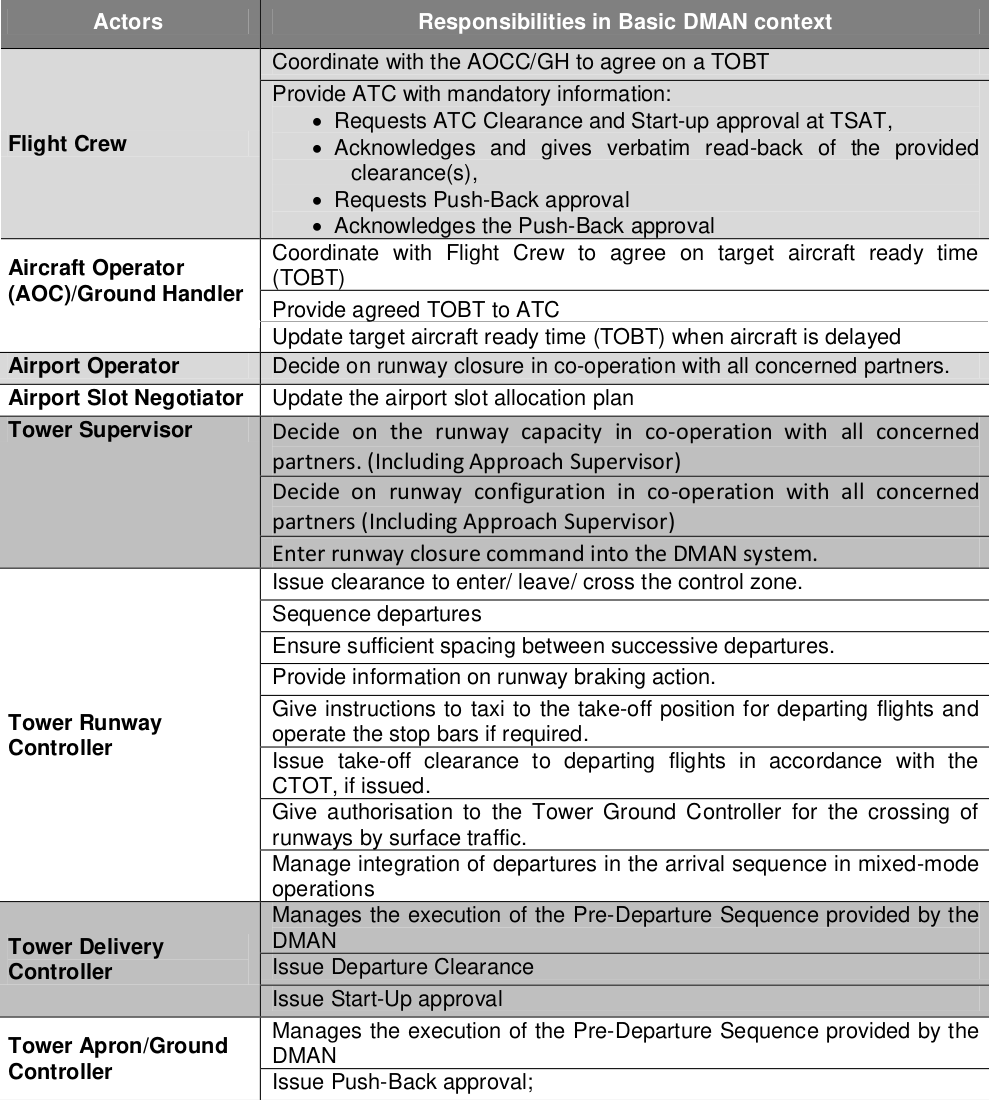
\includegraphics[width=9cm]{tabella.png}
	\caption{List of actors involved in turn around operations and their responsibility with respect to the DMAN system.}
	\label{actors}

\end{figure}

\bigskip
The table shows that there are 8 actors involved in the ground operations. One of the challenges of the ABM will be to simplify the complexity of interactions deriving from this organizational setting without losing accuracy.

\newpage
\part{Data Analysis}

The data analysis were performed on a data set provided by DGAC that contains information about 1059702 flights, that correspond to all the flights managed by CDG airport from 01/01/2018 to 29/02/2020.


\section{Exploratory analysis: Taxi time dependency on companies and associated stand}\label{exploratory}

One of the factors that could influence the pilots behavior, and consequently the taxi time, is the aircraft operator (air company). In fact, for example, we expect Air France pilots to be quicker in taxiing because they know the airport better. Another behavior that has been reported by CDG ATCOs is that Ryanair flights tended to declare to have run out of fuel to gain the priority in landing, even if it wasn't true. We tried to detect eventual inconsistencies in the taxi time for the most frequent users of CDG.

\subsection{Taxi time distribution for different companies}
Below is a plot of the histograms of taxi times for the 5 most frequent aircraft operators at CDG.

\bigskip
\begin{minipage}{\textwidth}
	\begin{minipage}[b]{0.5\textwidth}
		\centering
		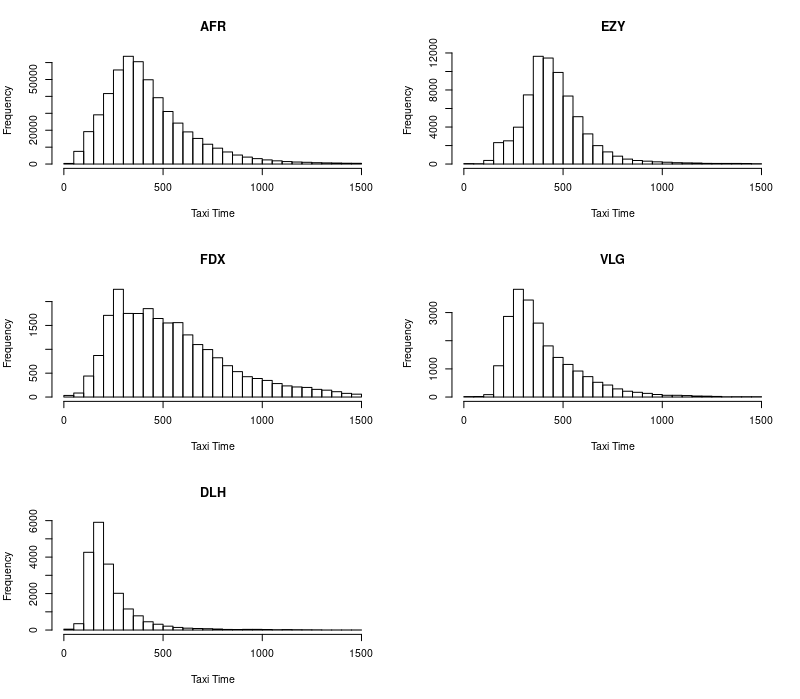
\includegraphics[scale=0.3]{companiesTaxiTime.png}
		\captionof{figure}{Histograms of taxi times for different companies at CDG.}
		\label{companiesFig}
	\end{minipage}
\hfill
	\begin{minipage}[b]{0.4\linewidth}
		\centering
		\tiny
		\begin{tabular}{p{0.8cm}p{1.3cm}p{0.8cm}p{0.6cm}}\hline
			Company & N° of flights over the total n° of flights & Mean Taxi Time(s) & $\sigma$ (s)\\ \hline
			AFR & 48\%& 433 s & 261 s\\
			EZY & 7\% & 460 s & 194 s\\
			FDX & 2\% & 548 s & 315 s\\ 
			VLG & 2\% & 403 s & 212 s\\
			DLH & 2\% & 240 s & 191 s\\
			\hline
		\end{tabular}
	\bigskip
	\bigskip
		\captionof{table}{Percentage over the total number of flights, avarage taxi time and relative standard deviation for the company whose flight are the most frequent at CDG.}
		\label{companiesTable}
	\end{minipage}
\end{minipage}
\bigskip

Figure \ref{companiesFig} and table \ref{companiesTable} show that different taxi times correspond to different companies.  

\subsection{Taxi time model}

Large taxi times can be caused by many events, like bad weather conditions, operational inefficiencies, aircraft malfunctioning, etc.. But in our approach to the data analysis, we decided to begin with a very simple model of taxi time, to identify which of the independent variables that the taxi time depends on is the major contributor.

The taxi time ($t_t$) can be modeled as ($t_t$):
\begin{equation}\label{time-eq}
t_t = \frac{d}{v} + t_{w}, 
\end{equation}
where $d$ is the distance traveled by the aircraft, $v$ is the aircraft speed, $t_{w}$ is the waiting time during taxiing.

As a first try, we tried to link the longer mean taxi time of some companies with the distance $d$.

\subsection{Taxi time VS taxi distance}\label{regression}
We performed a linear regression to verify the relation between the mean taxi time calculated over all the flights of a specific company and the respective mean taxi distance, that are shown in table \ref{tableDistances} for the most frequent user of CDG.

\begin{table}[h!!!!!!!!!!!!!!!!!!!!!!]
\centering

\begin{tabular}{p{1.5cm}p{1.5cm}p{1.6cm}}\hline
	Company & Mean Distance & Mean Taxi Time\\ \hline
	AFR & 3.22 NM & 433 s \\
	EZY & 3.30 NM & 460 s\\
	FDX & 3.78 NM & 548 s\\ 
	VLG & 3.03 NM & 403 s\\
	DLH & 2.32 NM & 240 s\\
	\hline
\end{tabular}
\captionof{table}{Mean taxi distance and mean taxi time for different companies.}
\label{tableDistances}
\end{table}

The linear regression gave the following result.

\begin{table}[h!!!!!!!!!!]
	\centering
	\begin{tabular}{p{1.5cm}p{1.5cm}p{1.5cm}p{1.4cm}p{1.7cm}}\hline
		 & Estimate & Standard Error& t value & p value ($Pr(>|t|)$) \\ \hline
		\smallskip Intercept & \smallskip -282.87 & \smallskip 34.93 & \smallskip -8.099s & \smallskip 9.18e-15\\
		 \smallskip Slope &\smallskip 244.32 &\smallskip 34.93 &\smallskip 21.526 &\smallskip < 2e-16\\

		\hline
	\end{tabular}

	\captionof{table}{Results of the linear regression.}
	\label{linearRegression}
\end{table}

Since the t value showed a statistically significant difference of our data with the null hypothesis, we can conclude that the differences in taxi times for the various companies are mostly due to the different distances traveled by the aircraft of these companies. 
In fact, at CDG a precise parking area in assigned, and some of them are more unfavorable than others in terms of taxi distance, as shown in section \ref{comparison}.


\subsection{Night time peak in taxi times}

If we plot the taxi time averaged over all the flights as a function of the hour of the day we see a peak that cannot be explained by the number of aircraft that are crossing the taxiway (Figure ~\ref{n_avions}).

\begin{figure}[h]
	\centering
	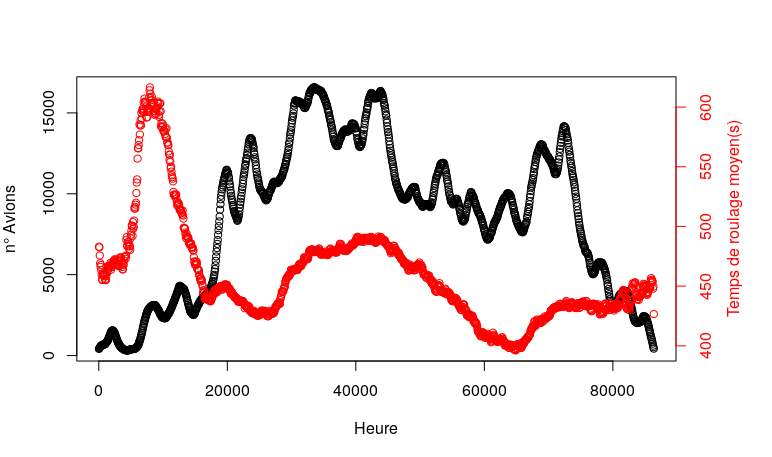
\includegraphics[width=8cm]{n_avions_TempsRoulage}
	\caption{Comparison between number of aircrafts in the taxiway (black line) and taxi time (red line).}
	\label{n_avions}
\end{figure}

So we performed an analysis of all the variables, included in equation \ref{time-eq}, that can contribute to the unexplained peak of 3 a.m

\begin{figure}[h!!!!!!!!!]
	\centering
	\begin{subfigure}[b]{0.5\textwidth}
		\centering
		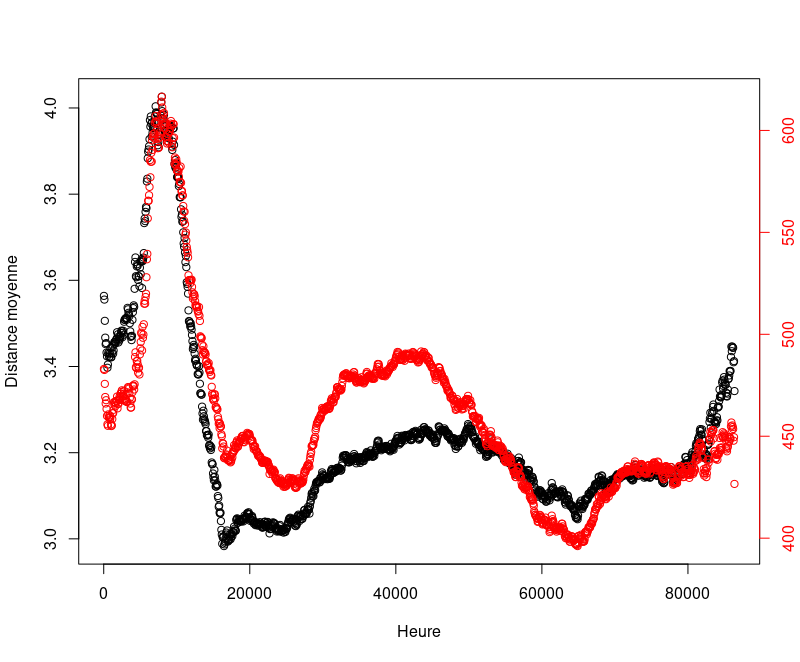
\includegraphics[width=5cm]{Distance}
		\caption{Comparison between distance of the parking from the runway (black) and taxi time (red).}
		\label{distance}
	\end{subfigure}
	\hfil
	\begin{subfigure}[b]{0.4\textwidth}
		\centering
		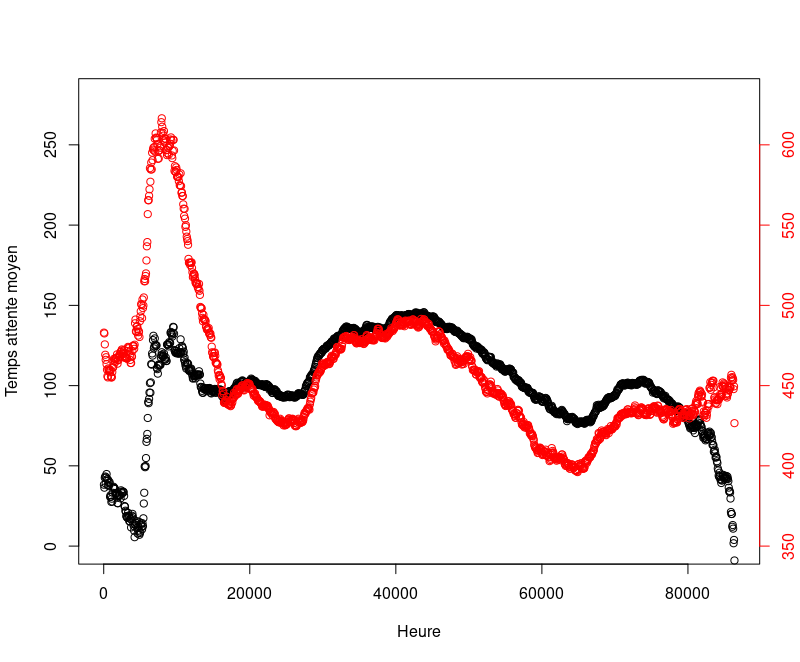
\includegraphics[width=5cm]{TempsAttente}
		\caption{Comparison between waiting time during the taxiing (black) and taxi time (red).}
		\label{waiting}
	\end{subfigure}
	\begin{subfigure}[b]{0.7\textwidth}
		\centering
		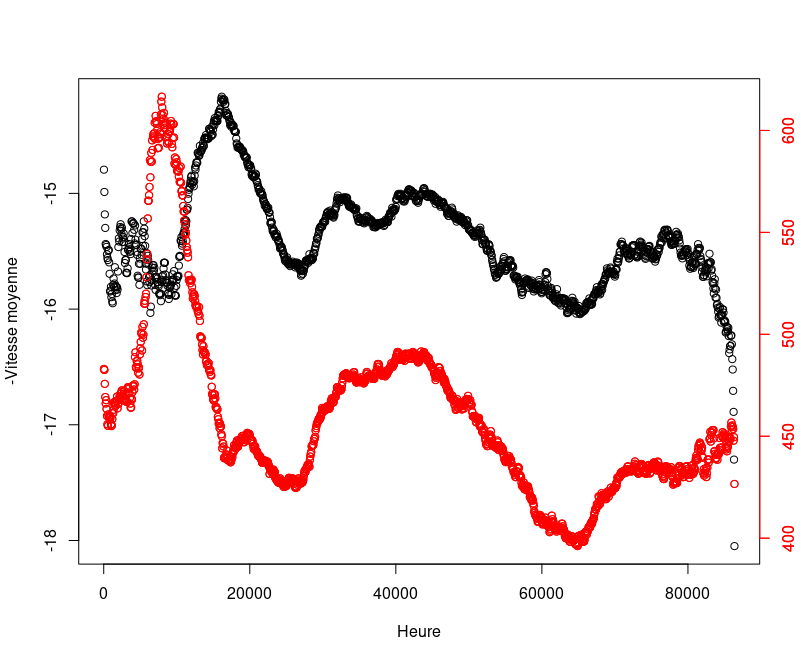
\includegraphics[width=5cm]{Vitesse}
		\caption{Comparison between the opposite (since we expect the taxi time to be inversely proportional to the speed) of average speed during the taxiing (black) and taxi time (red).}
		\label{vitesse}
	\end{subfigure}
	\caption{Behavior of average taxi time as a function of the hour of the day compared to the behavior of parking-runway distance, waiting time and speed.}
	\label{comparisons}
\end{figure}




As we can see from Figure \ref{comparisons}, what explains better the night time peak is the larger distance traveled by the aircraft on average at that hour. Also the waiting time gives a little contribution, while the speed is on average larger in correspondence of the peak. This means that it gives a negative contribution to the taxi time, with respect to the other hours of the day.

From an the interviews with the GC it emerged, in fact, that every night at least a couple of the four runways is closed, alternating the northern and the southern couple every 2 weeks. The runways stay usually closed from midnight to 5 a.m..
Then, the peak of 3 a.m. can be explained if the distance between the stand and the open runway is on average longer than during day time.

This hypothesis is verified in section \ref{comparison}.


\subsection{Comparison between AFR and FDX stands}\label{comparison}

We explored the dependency of taxi time on the runway and on the parking area, with a particular focus on Air France and FedEx flights. 

In fact, the length of the route from the stand to the runway explains not only the fact that the average taxi time for Fed-Ex is longer than the one of Air France, but also the night time peak. In fact, Fed-Ex flights occur usually at night, as shown in table \ref{companiesNight}.



\begin{table}[h!!!!!!!!!!!!!!!!]
	\begin{center}
		\caption{Average company frequencies for the whole day (left) and for the time interval 1:35 a.m. - 3.40 a.m. (right)}
		\label{companiesNight}
		\begin{tabular}{p{1.5cm}p{2cm}} % <-- Alignments: 1st column left, 2nd middle and 3rd right, with vertical lines in between
			\textbf{Company} & \textbf{Frequency whole day}\\
			\hline
			AFR & 48,3\% \\
			EJU & 6,8\% \\
			FDX & 2.25\% \\
		\end{tabular}
		\quad
		\begin{tabular}{p{1.5cm}p{2cm}} % <-- Alignments: 1st column left, 2nd middle and 3rd right, with vertical lines in between
			\textbf{Company} & \textbf{Frequency night time}\\
			\hline
			FDX & 26,8\% \\
			AFR & 26,4\% \\
			ABR & 20,3\% \\
		\end{tabular}
	\end{center}
\end{table}



We expect the taxi time to be larger when the distance between the parking slot and the runway is larger. This is especially evident with FedEx flight, since they all leave from the same parking area, situated at the periphery of the airport platform.

\begin{figure}[h]
	\centering
	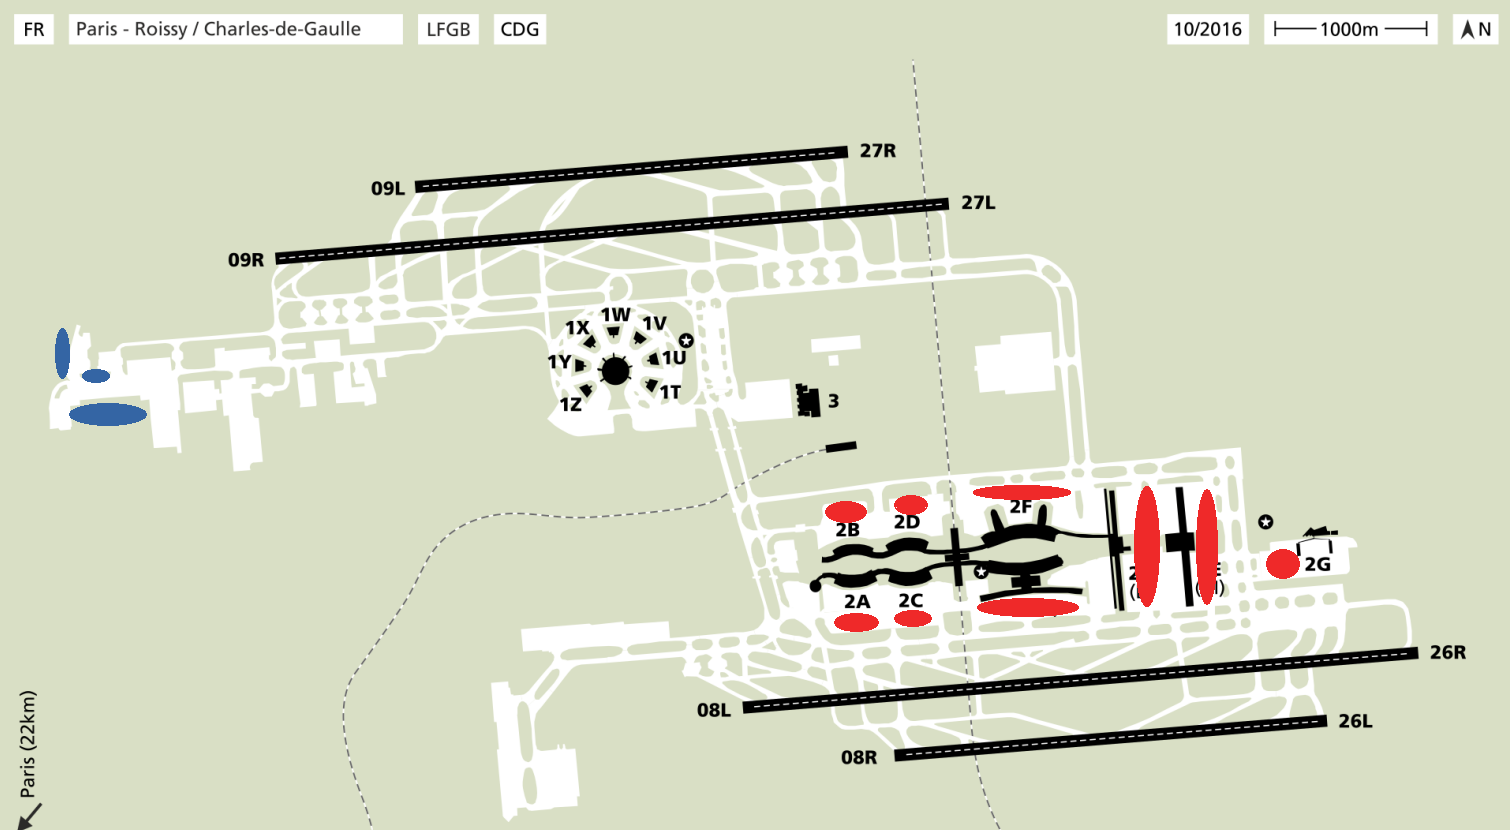
\includegraphics[width=\textwidth]{map_airport_filled}
	\caption{Map of Charles de Gaulle airport. The red ovals correspond to the gates where Air France aircraft usually park. The blue ovals correspond where FedEx aircraft park.}
	\label{map}
\end{figure}

Figure \ref{map} shows a map of the entire airport, where the parking areas for FedEx and AirFrance aircraft are evidenced.
We can see from the map that Air France aircraft have a quicker access to the runways, especially the southern ones ( runways 08L, 08R, 26L, 26R), since their parking position is central. FedEx aircraft, on the other side, have a quite quick access to the northern runways only when they are taking off facing east or landing facing west(runways 09R and 09L). While the large distance from the southern runways is the main reason for larger taxi times for FedEx flights.


\subsection{Conclusions and link with ABM}
We showed how the difference in taxi times showed in Figure \ref{companiesFig} can be explained at the first order with the distance between the stands associated with the companies and the runways. The results can explain also the night time peak showed in figure \ref{n_avions}.

The previous results have one main consequence in the implementation of the agent based model: the structure of the airport platform is fundamental to reproduce accurately the real taxi time distribution in our simulation.


\section{Current data analysis: detection of non-standard scenarios}\label{non-standard}
After an interview with the GC, we decided to focus on the detection of non-standard scenarios that occurred in the period of our data set.
In fact, what the GCs evidenced was that the main problems occur during high traffic hours and when non-predicted events occur. For the rest of the time, they follow standard procedures described in the ground booklet\cite{livret}.

In standard situation, the rules are followed and the algorithm describing the ground controller decision making process should be quite simple (even if even in standard scenarios they have some decisions to take, such as which entrance/exit to use to/from the runway).
What our current and future data analysis is focused on is the detection of non-standard situations, to be able to isolate them and perform an analysis on the behavior of the GC in these cases.

Below is a list of non-standard scenarios and a possible way to detect them in our data set.
\begin{itemize}
	\item \textbf{Closed taxiway.} They can be detected thanks to the feature ``Cheminement" of our data set, that lists all the main taxiways used by an aircraft during his taxiing procedure, in order. We expect that if a taxiway is closed, it won't be used during a certain time range by any aircraft, even if it is part of the standard path that should have been used.
	\item \textbf{Closed runway.} From an interview to the GC, it emerged that we can distinguish between closure at night time and at day time. At night time, one couple of the four runways is closed, alternating the northern and the southern couple every 2 weeks. At daytime, a runway can be closed for three main reasons: daily inspection(3 times a day, duration 10-20 minutes), inconveniences such as bird strikes (duration 10-30 minutes), technical work that needs to be done at daytime, linked to the radio electric system (duration 1-2 hours).
	
	Runway closure can be detected thanks to the creation of a new variable that represents the time interval between two flights that use the same runway. When this time is too long, the runway can be considered closed.
	\item \textbf{Bad weather conditions.} They can be detected integrating the weather data to our dataset (we asked the dataset to DGAC but they provided only for a dataset of 2 months).
	\item \textbf{De-icing procedures.} There is a variable called ``TempsDegivrage" in our dataset. It is necessary to understand how this variable impacts the eventual delay of flights.
\end{itemize}

Another way of proceeding is to isolate the flight of our data set with a too long taxi time and try to understand what causes it.

\subsection{Detection of runway closure}

We tried to detect the closure of a runway introducing a new variable in our dataset, that indicates the time interval between two consecutive usages of the same runway. To be noticed is the fact that the four runways are indicated with different names, according to the orientation with which they are used. In our analysis we treated as the same runway the couples 26R and 08L (south runway for departures), 26L and 08R (south runway for arrivals), 27R and 09L (north runway for arrivals), 27L and 09R (south runway for departures).

From the table below, we can notice that every day at least one of the four runways were closed for at least one hour, and in the 98\% of the days analyzed at least one runway have been closed for at least four hours, and within those days the majority closures happened from 11 p.m. to 5 a.m..
We see that for 4 times a runway were closed for more than one day. Looking at those data, what emerges is that the southern runway for departures were closed for 4 days from 14/11/19 to 18/11/19, while the southern runway for arrivals were closed for three months, from 07/07/18 to 09/10/18, with an interruption in the closure where a few aircrafts use the runway on 01/08/18 and 05/09/18.

\begin{table}[h!!!!!!!!!!!!!!!]
	\begin{tabular}{C{2cm}|C{2.5cm}|C{2.5cm}|C{2.5cm}}
		\textbf{Time interval (hours)} & \textbf{N of days of closure}& \textbf{N of days of night time closure} & \textbf{N of days of day time closure}\\
		\hline
		1 & 790 (100\%) & 789 (99\%)& 227 (35\%)\\
		2 & 789 (99\%)& 786 (99\%)& 112 (14\%)\\
		3 & 786 (99\%)& 783 (99\%)& 83 (10\%)\\
		4 & 777 (98\%)& 774 (97\%)& 65 (8\%)\\
		5 & 615 (77\%)& 591 (77\%)& 56 (7\%)\\
		6 & 221 (27\%)& 174 (26\%)& 52 (6\%)\\
		7 & 32 (4\%)& 17 (3\%)& 15 (1\%)\\
		24 & 4 (0,5\%)& 2(0,2\%) &2 (0,2\%) \\
	\end{tabular}
	\caption{Table of the occurrences of days in which a closure that lasted more than the time interval indicated in the first column happened. The third column indicates the number of days where the closure occured between 11 p.m. and 5 a.m., the fourth column between 5 a.m. and 11 p.m.. The total number of days analyzed were 790.}
\end{table}


Every flight in the data set is now labeled with the information wether a runway is closed or not. We consider a runway closed if it's not used for more that 30 minutes during daytime (from 6 a.m. to 12 a.m.) or for more than 4 hours during night time (from 12a.m. to 6 a.m.).

\subsubsection*{Further work}
We will have to perform a data analysis that shows the difference in the behavior of aircraft when a runway is closed.

\subsection{Research of the expected runway}

From the interviews with the GCs it emerged that the runway that a flight should use is chosen by the DMAN based on the strategy that the tower supervisor suggests to it. The strategy usually consists in choosing the runway based on the destination (in case of departures) or on the origin (in case of arrivals) to avoid crossings in the sky, since they are a lot more difficult to handle. 

We tried to verify this strategy. We grouped the flights based on their destination or origin, and looked at the percentage of flights that took off or landed from the northern runway and from the southern one, expecting to have extreme values. In fact, if the strategy used for choosing the runway is based on the destination/origin, we expect that almost 100\% of flights with the same destination take off/land on the same runway.

The data showed, on the contrary, that only for 55\% of departing flights to a same destination it is assigned the same runway more than 80\% of the time. For the other destinations, the runway is assigned following criteria that are different from the direction of the destination.

\subsubsection*{Further work}
Interview the tower supervisor or the GCs about the criteria used to choose a runway.

\subsection{Detection of the usage of non-standard taxi paths}

The GC booklet \cite{livret} contains a list of all the standard paths, that link every parking area to every runway. The data set provides for a variable ``Cheminement" that contains the sequence of taxiways used by the aircraft to go from the runway to the parking area and vice versa. Comparing the two, we can detect the cases when the standard path were not used, and use it as a proxy for unexpected events, such as taxiway closure, aircraft stuck on the taxiway, congestion, etc..

Something to be noticed is that the standard paths in the GC booklet contains only the main taxiway to follow, and not the runway entrance and exit to use, which remains at discretion of the ground controller (then, this decision has to be modeled in the ABM).

This analysis has to be completed and the results are not available yet.


\subsection{Issue in the inspection of long taxi time}

One of the strategies that could be used to analyze the causes of delays during taxiing is to isolate the flights with a long taxi time and try to detect the causes of it through the data. 

In particular, equation \ref{time-eq} shows that the main contribution to taxi times can be given whether by long distances, low speed or long/high number of waiting times.

These situations can in turn have different causes, that can be operational ones or physical ones. With the data analysis, we aim at detecting operational flaws, and with the ABM at simulating them and finding a solution to them. Physical causes, on the contrary, cannot be solved by the ABM.
Some examples of operational and physical causes of delay are showed in table \ref{causes} .
\begin{table}[h!!!!!!!!!!!!!!!]
	\begin{tabular}{|p{3cm}|p{4cm}|p{4cm}|}
		\hline
		\textbf{Event}& \textbf{Operational causes}& \textbf{Physical causes} \\
		\hline
		Long distances & An aircraft that took the wrong way has to go back, increasing the distance traveled & The stand is far from the runway \\
		\hline
		Low speed & A pilot decides to travel at low speed & Safety constraints in low visibility conditions\\
		\hline
		Long waiting times during taxiing & A potential crossing hasn't been detected soon enough and one aircraft is forced to stop to give way to the other; 
		
		An aircraft is stuck in the taxiway and an alternative path for other aircraft hasn't been elaborated quickly enough & An aircraft gets stuck in the taxiway due to some malfunction \\
		\hline
		Long waiting times at the runway & The runway capacity hasn't been accurately computed, addressing too many aircraft to it & Runway closed\\
		\hline
	\end{tabular}
	\caption{Examples of operational and physical causes of long taxi times.}
	\label{causes}
\end{table}

From the table, we can notice that the same measurable phenomenon can have really different causes. It's really difficult 

TODO

\newpage


\part{Interviews}
Thanks to the interviews with the GC and the pilots, we are able to describe in detail their job and their influence in the taxi time

\section{Ground Controller}

\subsection{Organization of the work}
\paragraph{Geographical splitting:}There are three control towers where the ground controller can work: southern, northern and central. The central tower is used at night, from 10 pm to 6:30 am, and at most 3 ground controllers can work there at the same time. The southern and northern towers are used during day time, and at most 2 ground controllers can work at the same time in each of the two tower. So, during daytime there can be at most 4 ground controllers working at the same time.

During daytime, there are 4 PAI (point d'arret intermediaire) between the northern ground and the southern ground: Middle1 (taxiway N), Middle2 (F), Middle3 (B) and Middle4 (Q). Those points are the borders between north sector and south sector.

Some tasks are different between the north and and south. For example, GCs on the north part have to handle with push-backs when there are some specific apron controllers who do that for the south part of the field (in fact from 10pm to 7am, there is no apron controller and the GCs have to handle it also on the south). 

In the northern (southern) tower, there is a ground controller always working, and a backup ground controller that begins to work whenever the first GC choose to split his sector in two. Each sub-sector is covered by one specific radio frequency. When the ground controller works on the full northern(southern) sector, he or she merges the two radio frequencies.

In same room of the ground controllers, we can also find the delivery controller and the runway controller workstations. The apron controller and the tower supervisor work in separate rooms.

\paragraph{Working shift:} In an 8 hour shift, there is a team of 2 or 3 ground controllers working for each tower. Each one of them is in charge of the traffic for one hour, then they have a break for another hour. During the break, they have to be ready for a split, in case the ground controller in charge needs it, or to answer to the phone calls coming from other controllers, if they notice that their colleague can't handle them alone. 


\subsection{Tasks}

GC job is leading an aircraft safely from the apron area to the runway entrance. 

What he is in power of deciding is:
\begin{itemize}
	\item the taxi route for the flights;
	\item the moments and the place where aircraft have to stop during taxiing, for example to give way to another aircraft;
	\item the runway entrance;
	\item the sequence of departures at the holding point;
	\item a change of runway in agreement with the supervisor and the pilot.
\end{itemize}

\subsection{Tools}
To take his decisions, the GC takes into consideration different information, that he gains through his tools and through the communication with other controllers and airport actors.

The tools he uses are the following:

\begin{itemize}
	\item \textbf{Ground radar screen.} It contains an interactive map of CDG airport platform (it is possible to zoom in and out). The GC usually chooses to zoom on its sector, but to keep an open window on other sectors to be able to anticipate if an aircraft is directed towards his sector.	
	On the map, the position of each aircraft on the platform is constantly updated. To each aircraft position is associated its identification code, speed and aircraft type, through a tag over the position of the aircraft.
	The blue tags are for departures, the red ones are for arrivals. The blue tags appear on the screen a few minutes before the push back.
	\item \textbf{View.} The information about aircraft position is gained by direct sight, too.
	\item \textbf{Paper strip.} In front of the GC there is a wooden holder that can host 20 paper strips. Each paper strip corresponds to an aircraft that the ground controller has to handle. Some important information is already written on the strip when it's printed, and some other information is added by the GC.
	In particular, when it's printed we can find: the aircraft ID, the type of departure, runway of departure, stand number. Furthermore, arriving aircraft and departing aircraft can be distinguished by the color of the strip (blue for departures, white for arrivals). 
	The GC will add: the proposed holding point at the runway, the path.
	
	The ground controller places the strips on the wooden carrier in positions that help him remind the priorities of the various aircraft.
	
	The strips are printed 10-15 minutes before the aircraft lands in case of arrivals, as soon as the delivery controller gives the permission for the startup, usually 10 minutes before the startup, in case of departure.
	
	\item\textbf{Sky radar screen.} It shows the position of aircraft that are flying around the airport.
	\item\textbf{Frequency regulator.} It allows to transmit, monitor and group frequencies.
	\item\textbf{Radio.} It is used for communications with the pilots.
	\item \textbf{Phone.} It is used for communications with the controllers that are not in the same tower.
	
	
\end{itemize}



\subsection{Communication}
\subsubsection*{Ground controllers}
In order to coordinate the work of ground controllers, they use to exchange a lot of information. They can do it directly or by using their phones, if it is easier. They are exchanging information about current planes, potential sources of traffic's complexity or incoming strategy.

\subsubsection*{Runway controller}
The RC and the GC do not communicate if not necessary. The standard procedure is described below:

\textit{Arriving aircraft}: the runway controller tells the pilot to set the frequency on Ground Control once the aircraft has crossed the departure runway (in fact, because of the configuration of runways, an arriving aircraft has always to cross the departure runway to get to the stand). 
He is in charge of deciding the exit taxiway from the runway.


\textit{Departing aircraft}: in standard situations, the GC just passes the paper strip containing all information about the aircraft to the runway controller when it's the right time.
\\

When the situation requires it (often in rush hours) they exchange the following messages:
\begin{itemize}
	\item (From RC to GC)The runway controller can change the holding point decided by the ground controller if he says it early enough. He can ask for a change of holding point up to the moment when it's not possible for the ground controller to warn the pilot in time, so also 2 minutes before the aircraft gets to the holding point. But he usually does it when the aircraft is far away, for example when there is an aircraft stuck at the holding point.(Ex. ``\textit{I've got a stuck aircraft on Q4, can you please put AFR123 on Q5?}")
	
	\item(From GC to RC)The GC always has to explicitly communicate to the runway controller when he's not using an usual entrance to the runway, to avoid accidents. 
	
	\item(From GC to RC) The GC warns the RC if an arriving aircraft is late, so that the RC can make it cross the departure runway instead of start a take off (Ex. ``\textit{AFR123 needs to be at the stand in 5 minutes, can you give it the priority?}")
\end{itemize}


\subsubsection*{Delivery controller}
The RC and the GC do not communicate if not necessary. There can be two main reason for speaking with the delivery controller:
\begin{itemize} 
	\item The GC is contacted by a pilot asking for a push-back ealier than the TSAT. He or she then calls the delivery controller to check if it's ok to push-back. 
	\item The GC is contacted by a pilot who has a problem and will not be able to start a the planed hour, so he or she calls the delivery controller to put back the flight in the DMAN (that will re-calculate the TSAT).
\end{itemize}
\subsubsection*{Apron controller}
In nominal situation there is no communication as long as standard procedures are respected. The GC only tells to pilots to change the frequency.
\\
In low traffic condition, they may not communicate conditions even if the GC chooses a non-standard PAI: if the pilot is asked to change his frequency soon enough, the apron controller has the time to realize that he's receiving an aircraft at the wrong PAI.
\\
When the situation requires it (really often in peak hours) they exchange the following messages:

\begin{itemize}
	\item When there is an aircraft arriving and one leaving the apron area, so it's not clear who has the priority.
	\item (GC to AC as well as AC to GC) GC or AC needs to use a PAI which is not the standard one. (Ex. Apron to Ground:\textit{"I'd like to put AFR123 on TA2, is it ok for you?"``no, there is a tugged aircraft crossing that way"} or Ground to Apron:\textit{"\textit{Is it ok if I pull AFR123 on TE3}?"``No, I've got a push back there, go to TE2"})
\end{itemize}


\subsubsection*{IFR room}
This interaction does not happen often, and it usually passes through the supervisor. A GC can make the following requirements when there are some serious traffic issues:
\begin{itemize}
	\item reroute an aircraft to another runway;
	\item make an aircraft wait in the sky.
\end{itemize}

\paragraph{Ground handling services:}
It's usually the tower supervisor that handles the communications with ground handling services. They could be called:
\begin{itemize}
	\item to ask for a tug;
	\item to ask for the opening of a deicing bay.
\end{itemize}

\subsubsection*{Pilots}
Pilots can not do something without the clearance gived by the GC. 
They are talking together by radio, using the frequency that covers this geographical part of the field. Between each section pilots have to change the frequency they are using and wait to get in touch with the new GC before carrying on their taxiing. 

The GC can give a total or partial clearance to pilots. In particular, we can distinguish different kinds of messages based on if the aircraft is arriving or departing.

\textbf{Arrivals}: the runway controller gives the clearance to land or to stay in the sky and the clearance to cross the inner runway or to stop at the waiting point. When the pilot is about to finish the crossing calls the ground controller(Ex.pilot:"\textit{AFR123. We are crossing runway 27L at D6.}). There are several possibilities here:

\begin{itemize}
	\item the GC doesn't answer because he's too busy handling the other aircraft. In this case the aircraft stops.
	\item the GC answers but doesn't have time to give the clearance, so he just says that he'll call back. In this case the aircraft stops (Ex. GC: ``\textit{AFR123, I'll call you back}").
	\item the GC gives the clearance only about the first move (ex. turn left) and he calls back later (Ex. GC: ``\textit{AFR123, turn left and I'll call you back}").
	\item There are not many aircraft in the sector handled by the GC, so he will give the whole clearance, until the stand or until Middle1(2,3,4) (Ex. GC: ``\textit{AFR123, turn right on D and left on F, stop at Middle2}").
	\item There are many aircraft in the sector so the GC is not able to give the whole clearance, but only a partial one. The partial clearance includes the instruction to hold at a certain point in the taxiway, or to give priority to another aircraft (Ex. GC: ``\textit{AFR123, turn left on D and right on F, then hold short at B}" or ``\textit{AFR123, turn left on D then give way to AFR456 from your right}").
	\item In bad weather condition, the GC have to change the clearance they give because the pilots cannot see the other aircraft on the platform(Ex. they cannot say ``\textit{AFR123, turn left on D then give way to AFR456 from your right}", but they have to say ``\textit{AFR123, hold short at E}")
\end{itemize}

\textbf{Departures}: the GC has to handle the aircraft from the pushback, if there are no apron services in his sectors. If there is the apron service, the GC receives the aircraft at the PAI. 
In the first case, the GC gives the permission to push back (Ex. GC: ``\textit{AFR123, push back is approved facing west, call me back for taxi}" or ``\textit{AFR123, give way to the traffic rolling behind you and then push back is approved, call me back for taxi}" or ``\textit{AFR123, push back approved, could you make a long one to give way to AFR456 to roll ahead of you}"). 

Then, the aircraft is ready for taxi. At this point the GC has to give the clearance. The clearance arrives until the last point included in the GC sector (which could be the holding point or Middle1(2,3,4)). The clearance could be total or partial, as in the arrival case.
\subsection{Strategy}
\subsubsection{Path strategy}
The interviews with the GC showed that their strategy can be modeled in completely different ways, according to the situation. In particular, identified the following scenarios, associated to the respective behavior:

\begin{itemize}
	\item \textbf{High traffic scenario.} Up to four GC work at the same time in the control tower, each one of them checking over one portion of the airport platform. The GC follow the standard taxiways as much as possible. Their strategy is then well defined, and it should usually lead to predictable outcomes. 
	The rules that GC must keep in mind include the following examples \cite{livret}.
	\begin{itemize}
		\item Large aircraft cannot travel along some specific taxiways for safety reasons.
		\item Every parking area has some strict rules that regulate the entrance and the exit of aircraft (one way routes, etc.).
		\item A standard path is associated to every couple \textit{Parking Area, Runway}.
		\item The direction of one way taxiways changes based on the orientation of the runway (face east or west).
	\end{itemize}
	In this scenario, there are few reasons why a GC may deviate from the standard taxiway:
	\begin{itemize}
		\item an unusable taxiway (closed or work in progress or an aircraft stuck in it);
		\item holding points strategies (change the order at the holding point);
		\item priority strategies;
		\item splitting sectors strategies (if the colleague needs an aircraft in a specific taxiway because the alternative taxiway is too busy, even not using the standard direction);
	\end{itemize}
	\item \textbf{Low traffic scenario.} This situation happens at night, when one of the two couples of runways is closed. Only one GC is operating, and he controls the whole airport platform. The GCs can decide not to follow standard taxiways to gain some seconds in taxi times, since there is no danger of accident with other aircraft.
	
	\item \textbf{Non-standard scenario.} It's the case of bad weather conditions, aircraft stuck in the middle of the taxiway, unexpected runway closure, taxiway closure etc. Expecially in rush hours, the workload for GC in those cases is really high, since they have to think about a solution in a small amount of time. The strategy here is not well defined.
\end{itemize}

\subsubsection{Holding point strategy}
The taxiway used determines the length of the runway, that has to match the aircraft performance. The pilots make a performance computation for each entry, this way they can set up the engine and the take off speed. 

Usually, the standard entrances are used. Those taxiways can be chosen by GC without warning the pilot in advance. There are 2 standard entrances: the one that corresponds to the shortest runway is used for the medium aircraft, the other is used for the wide body aircraft. What happens with the interaction with the pilot is that the GC proposes an entry and if the pilot doesn't complain, it's a deal.

There are a few cases in which the standard procedures are not followed. 

For example, if an aircraft is traveling on a taxiway parallel to the runway, but in the opposite direction of the runway flow, the GC may choose the entrance that makes the runway the shortest possible, to reduce the taxi time. When they assign a non-standard taxiway, they have to provide for the length of the runway in their clearance. They have to propose it to the pilot in advance and he has to agree or not, or it can happen the opposite: the pilot proposes it (maybe because he wants to avoid the queue on the standard taxiways) and the GC has to agree. For example, Lufthansa flights are park at the north of terminal 1, and the aircraft is usually not big because they go to Germany. They often request Q2 (entrance with shortest runway) to be quicker in the taxiing and to avoid the queue in Q4 and Q5 (standard entrances).

Another example of non standard procedure is when the GC has to deal with aircraft of different types, one after another. In fact, in this case there are safety constraints on the time between two consecutive flights because of the wind turbulence generated by the first one. For example, if a medium aircraft departs right after a heavy aircraft from the same taxiway, it will have to wait at least 2 minutes. If it uses a taxiway that makes the runway shorter, it will have to wait 3 minutes.
\subsection{Human factor}
Every decision of the ground controller may influence the taxi time of an aircraft. The most evident one is the choice of a taxi route, but other important decisions may be the order in which deliver the messages to the pilots in case they are more than one at the same time, the priority strategy in case of conflict, the holding point strategy, the decision to split, the promptness in dealing with a problem or an emergency.

From the interviews with the GC, what they consider fundamental to handle efficiently the traffic are the following factor.
\begin{itemize}
\item \textbf{Splitting.}The splitting of the work is an decision which has some important effects on the taxi time. When the GC choose to split the area, the communication between him and the beackup GC becomes essential because he has to give instructions about the current state of traffic. But at the same time, he has to give instructions to planes he is in charge of, listen to them, think about his strategy, and speak to other controllers. Moreover, between two sections, planes have to stop to ensure the security.
\\
Accomplishing the splitting procedure takes approximately five minutes.

\item \textbf{Shift of GC in the workstation.}
Another event that can cause a lengthening of the taxitime is the arrival of a new GC. The current GC has to give information about the traffic, the weather, the tools' condition and, at the same time, continue following the planes.\\
Moreover, according to the time available for the current and the new GC, the change can be quite brutal. In high workload situation it can be difficult to handle.

\item \textbf{Frequency change.}
The first reason why an aircraft slows down or stops is because he's not receiving orders from the ground control. This happens especially when the pilot has to change frequency when he enters a new sector (from east to west or from north to south and vice versa): if the new GC isn't quick enough in giving the clearance to the new aircraft, the pilot will stop at the PAI.
How does the switch between frequencies happens? The first ground controller, that has taken care of the aircraft until the PAI, tells the pilot to switch the frequency at that point, to be able to speak with the new ground controller. It can happen that the GC does not warn the pilot in time, and the pilot crosses the PAI and continues taxiing without changing the frequency also for 500 m, until he's told to change. This happens once or several times a day, and it is a safety issue.

\item \textbf{Priority strategy.}
The aircraft may face other aircraft while he uses the assigned path. In this case, the ground controller has to give the priority to one of the two based on the slot, type of aircraft.

\item \textbf{Apron Area Management.}
Especially in terminal 1, which is the oldest and less efficient terminal in terms of traffic, you could have issues of priority between arriving and departing aircraft. A case that often happens is that an aircraft cannot enter the taxiway A in terminal 1 because another aircraft is pushing back, occupying the taxiway. In this case, one of the two has to stop (pushing back or entering the apron area). The same happens in terminal 3, where there is only one way for entering and exiting. 

\end{itemize}

\subsubsection*{Workload}
The most important concept related to the human factor that came out form GC interviews is the workload. The efficiency of the performance of GC is heavily influenced by it.

High workload in fact can prevent the GC to think about the best decision in terms of time optimization: he may choose the standard path instead of a short cut because he doesn't have time to think about an alternative path, he may tell a pilot to wait in the middle of the taxiway because he has no time to monitor his travel, he may choose a non-optimal sequence at the holding point.

What creates a high workload for the GC is the complexity of the traffic.
It depends heavily on the number of sectors the GC handles. There are three possibilities: night time (all the sectors merged), day time in a nominal traffic (north or south par of the field) and peak hour (only a quarter of the field). The complexity depends also on the sector itself. Below a list of situation that increase the complexity of the traffic and that depend or not on the sector in which the GC is working.



\newpage
\part{Agent Based Model}

\section{Current and new agent based model}

The model we developed during the first period of the project is quite simple, and it involves only aircraft agents.

We start with a single runway, 2-terminal airport. Aircrafts arrive at the runway from Terminals 1 and 2, located at distances $d_1$ and $d_2$ from the runway. At each terminal, there is a fixed schedule of departures (eg one plane departs every n time steps). However, this schedule is subject to random variations: each departure time is blurred by some random noise $\eta_i$ (the noise may be depend on Terminal because of gate design / architectural constraints / airlines operating there etc.). On their way from the gate to the runway, aircrafts move at constant speed $v$, so that from Terminal $i$, it takes them a time $t_i = d_i/v$ to get to the runway. However, on their way, they might incur an exponentially distributed delay $\delta_i$. When they arrive at the runway, aircraft enter a queue. With probability $p$, the first aircraft up the queue may have to wait because of inbound traffic (another plane landing). If so, the waiting time is exponentially distributed, with parameter $\lambda$. 
When the first aircraft in the queue takes off, then the next one may either take off immediately afterward, with probability $1-p$, or again, with probability $p$, have to wait because of inbound traffic. 
\smallskip

The model just described is basically a queuing model. When the demand (aircraft arriving at the runway) exceeds the runway capacity, a peak in waiting times at the runway is obtained. This peak partly reproduces the larger waiting time that we have on average during rush hours. 

But given the complexity of the airport platform, this model isn't sufficient. Moreover, it doesn't take advantage of the strength of agent based models, that is the possibility of modeling heterogeneous agents to see if the interaction between them leads to some emergent behaviors of the system.

We would like to build a model in which detailed structural information, namely the airport taxiway structure, are integrated with human/operational factors, namely the strategy followed by the agents involved in the taxiing operations. The main agents of the simulation are going to be the pilots/aircraft and the ground controllers, but other agents could be included (see section  \ref{other-agents}).


\subsection{Airport structure}

We decided to include a detailed simulation of the airport structure because of the results showed in section \ref{exploratory}. In fact, the mean of the distribution of taxi times depends on the distance traveled by the aircraft, therefore by the position of the stand and of the runway. The airport platform can be modeled as a network whose nodes are the parking areas and the intersection between taxiways, while the edges are the taxi routes. The weight of the edge is going to be equal to the route's length.

In an advanced version of the simulation, it could be interesting to include also the slopes of the taxiways, since they seem to produce emergent congestion phenomena (i.e. the slope towards south on the taxiways at the south east part of the airport platform, E, R, T).

To build this kind of network, we are going to use the AUTOCAD data provided from the airport.

\subsection{Ground Controller}

For the ABM, it is important to try giving a definition of workload. The workload can be measured by the number and importance of messages a GC has to deliver. The more messages a GC has to pass on, the less time is available to think about his or her strategy. At most, a GC can deliver around 6-7 messages\footnote{Pilots have to confirm that they received the message by repeating it so it doubles the length of a message.} per minute during a period a 10-15 minutes (it would be to difficult to carry on on that tempo during a longer period). 

\subsubsection{Pilots}

Another important agent is the pilot, that will maybe be merged with the agent aircraft to make the model simpler. 

The pilots have the task to inform the controllers when they are ready to push back, to obtain the clearance to begin the push back by the delivery controller.

From the interviews with GCs, it emerged that once the taxiing has begun the pilots have little autonomy while taxiing, since they have to follow the path indicated by ground controllers.
Nevertheless, they have the autonomy to choose the speed of taxiing.


\subsection{Doubts: operational range of the simulation and other agents}\label{other-agents}
The complexity of the airport system detailed in section \ref{ACDM} requires a special regard in the choice of the operational range described by the simulation, and of the list of agents involved.

There are many factors that can influence the taxi time. For departures: the schedule of TOBT (decided months before by the aircraft operators and the airport), the TSAT outputted by the DMAN 45 minutes before the push back, the runway chosen by DMAN, the runway capacity that the tower supervisor gives as an input to the DMAN. For arrivals: the time at which the aircraft receives the clearance to land, the availability of stands. For both: the path chosen by GC, the strategy of the GC in response to unexpected events.
Therefore, it is essential to define an operational range that we want to simulate in our ABM, and consequently the list of agents that we want to use. 

In fact, if we decide to improve the TSAT and the parameters given as an input to the DMAN, it is essential to include in our model a DMAN agent, a delivery controller that receives its output and gives the departure clearences, and a tower supervisor agent who set the parameters of the DMAN.

If we chose to focus on the strategy of GC, we will set as parameters the output of DMAN and the tower supervisor decisions about the input parameters of the DMAN. 
In fact, choosing this option we would make the simulation "blind" to what happens to the aircraft before it crosses the PAI and after it arrives at the holding point at the runway, and vice versa. Information about what happens in those time period arrive as a parameter to the GC, and not as an effect of the simulation. 

If we include in the simulation also what happens in the apron area (push-backs that prevent other aircraft to pass, miscommunication between the delivery controller and the pilot, etc.) and at the runway or in the sky (for example, an aircraft that gains precedence because it declares to have run out of fuel), we will need to model the apron controller, the runway controller and the approach controller, with which the GC interact. 

To take this decision, it is essential to understand what are the agents that the GC interact with and what is their role in the taxi time.



\begin{thebibliography}{9}
	
	\bibitem{gotteland}
	J.B. Gotteland,
	\textit{Optimisation du trafic au sol sur les grands aéroports,}
	PhD thesis,Institut National Polytechnique de Toulouse, 
	2004
	
	\bibitem{rathinam}
	S. Rathinam, J. Montoya, and Y. Jung, 
	\textit{An optimization model for reducing aircraft taxi times at the Dallas Fort Worth International Airport,}
	Proceedings of the 26th International Congress of the Aeronautical Sciences, 
	2008
	
	\bibitem{chua}
	Zarrin  K  Chua,  Mickael  Causse,  Mathieu  Cousy, Fabien  André,
	\textit{Modulating   Workload   for   Air   Traffic   Controllers   during   Airport Ground  Operations},
	Human  Factors  and  Ergonomics  Society Annual Meeting,  Oct  2015,  Los  Angeles,  United  States.  59  (1),  pp.16-20 Proceedings  of  the  Human  Factors  and  Ergonomics  Society  Annual Meeting, 
	2015
	
	\bibitem{noortman}
	T. Noortman,
	\textit{Agent-Based Modelling of an Airport’s Ground Surface Movement Operation: Understanding the principles and mechanisms of decentralised control,}
	2018
	
	\bibitem{ACDMimpact}
	EUROCONTROL,
	\textit{A-CDM Impact Assessment}, 
	2016
	
	\bibitem{DMAN}
	DMAN project partners,
	\textit{Basic DMAN Operational Service and Environment Definition (OSED)},
	2011
	
	\bibitem{livret}
	DGAC \& DSNA,
	\textit{Livret Sol CDG},
	2018
	
	\bibitem{manual}
	EUROCONTROL, ACI, IATA,
	\textit{Airport CDM Implementation Manual},
	2017
\end{thebibliography}
	
	
\end{document}